
\section*{Problem 2: Report on Player 15411's Outfield Defense}
\label{sec:expts}

The following evaluation is based on 375 hits for which player 15411 (henceforth, "the player") was identified as the primary fielder. The player's only recorded position for these 375 hits is center field.

The player began the 2023 season at level B and was transferred to level A about a month later (on May 5, 2023). The player was responsible for 237 air outs over the course of the season.

\subsection{Bottom Line Up Front}

\subsection{Overall Performance}
\label{sec:overallperformance}

The player's outfield performance during the 2023 season was in the 83rd percentile among qualified outfielders (at least 10 air outs during the season) in terms of mean air outs above expected (mAOAE). This statistic represents how much more likely a player is to catch a given ball than the average player. The player had a mAOAE of 0.026, so they were about 2.6 percentage points more likely to catch a given ball than the average player.

That said, this number conceals significant variation in the player's performance based on the type of ball which was hit into center field. As shown in Figure \ref{fig:hittype}, the player was significantly above average at catching hits classified as a barrel or solid contact, and below average at catching hits classified as a flair or burner.

\begin{figure}[htb]
    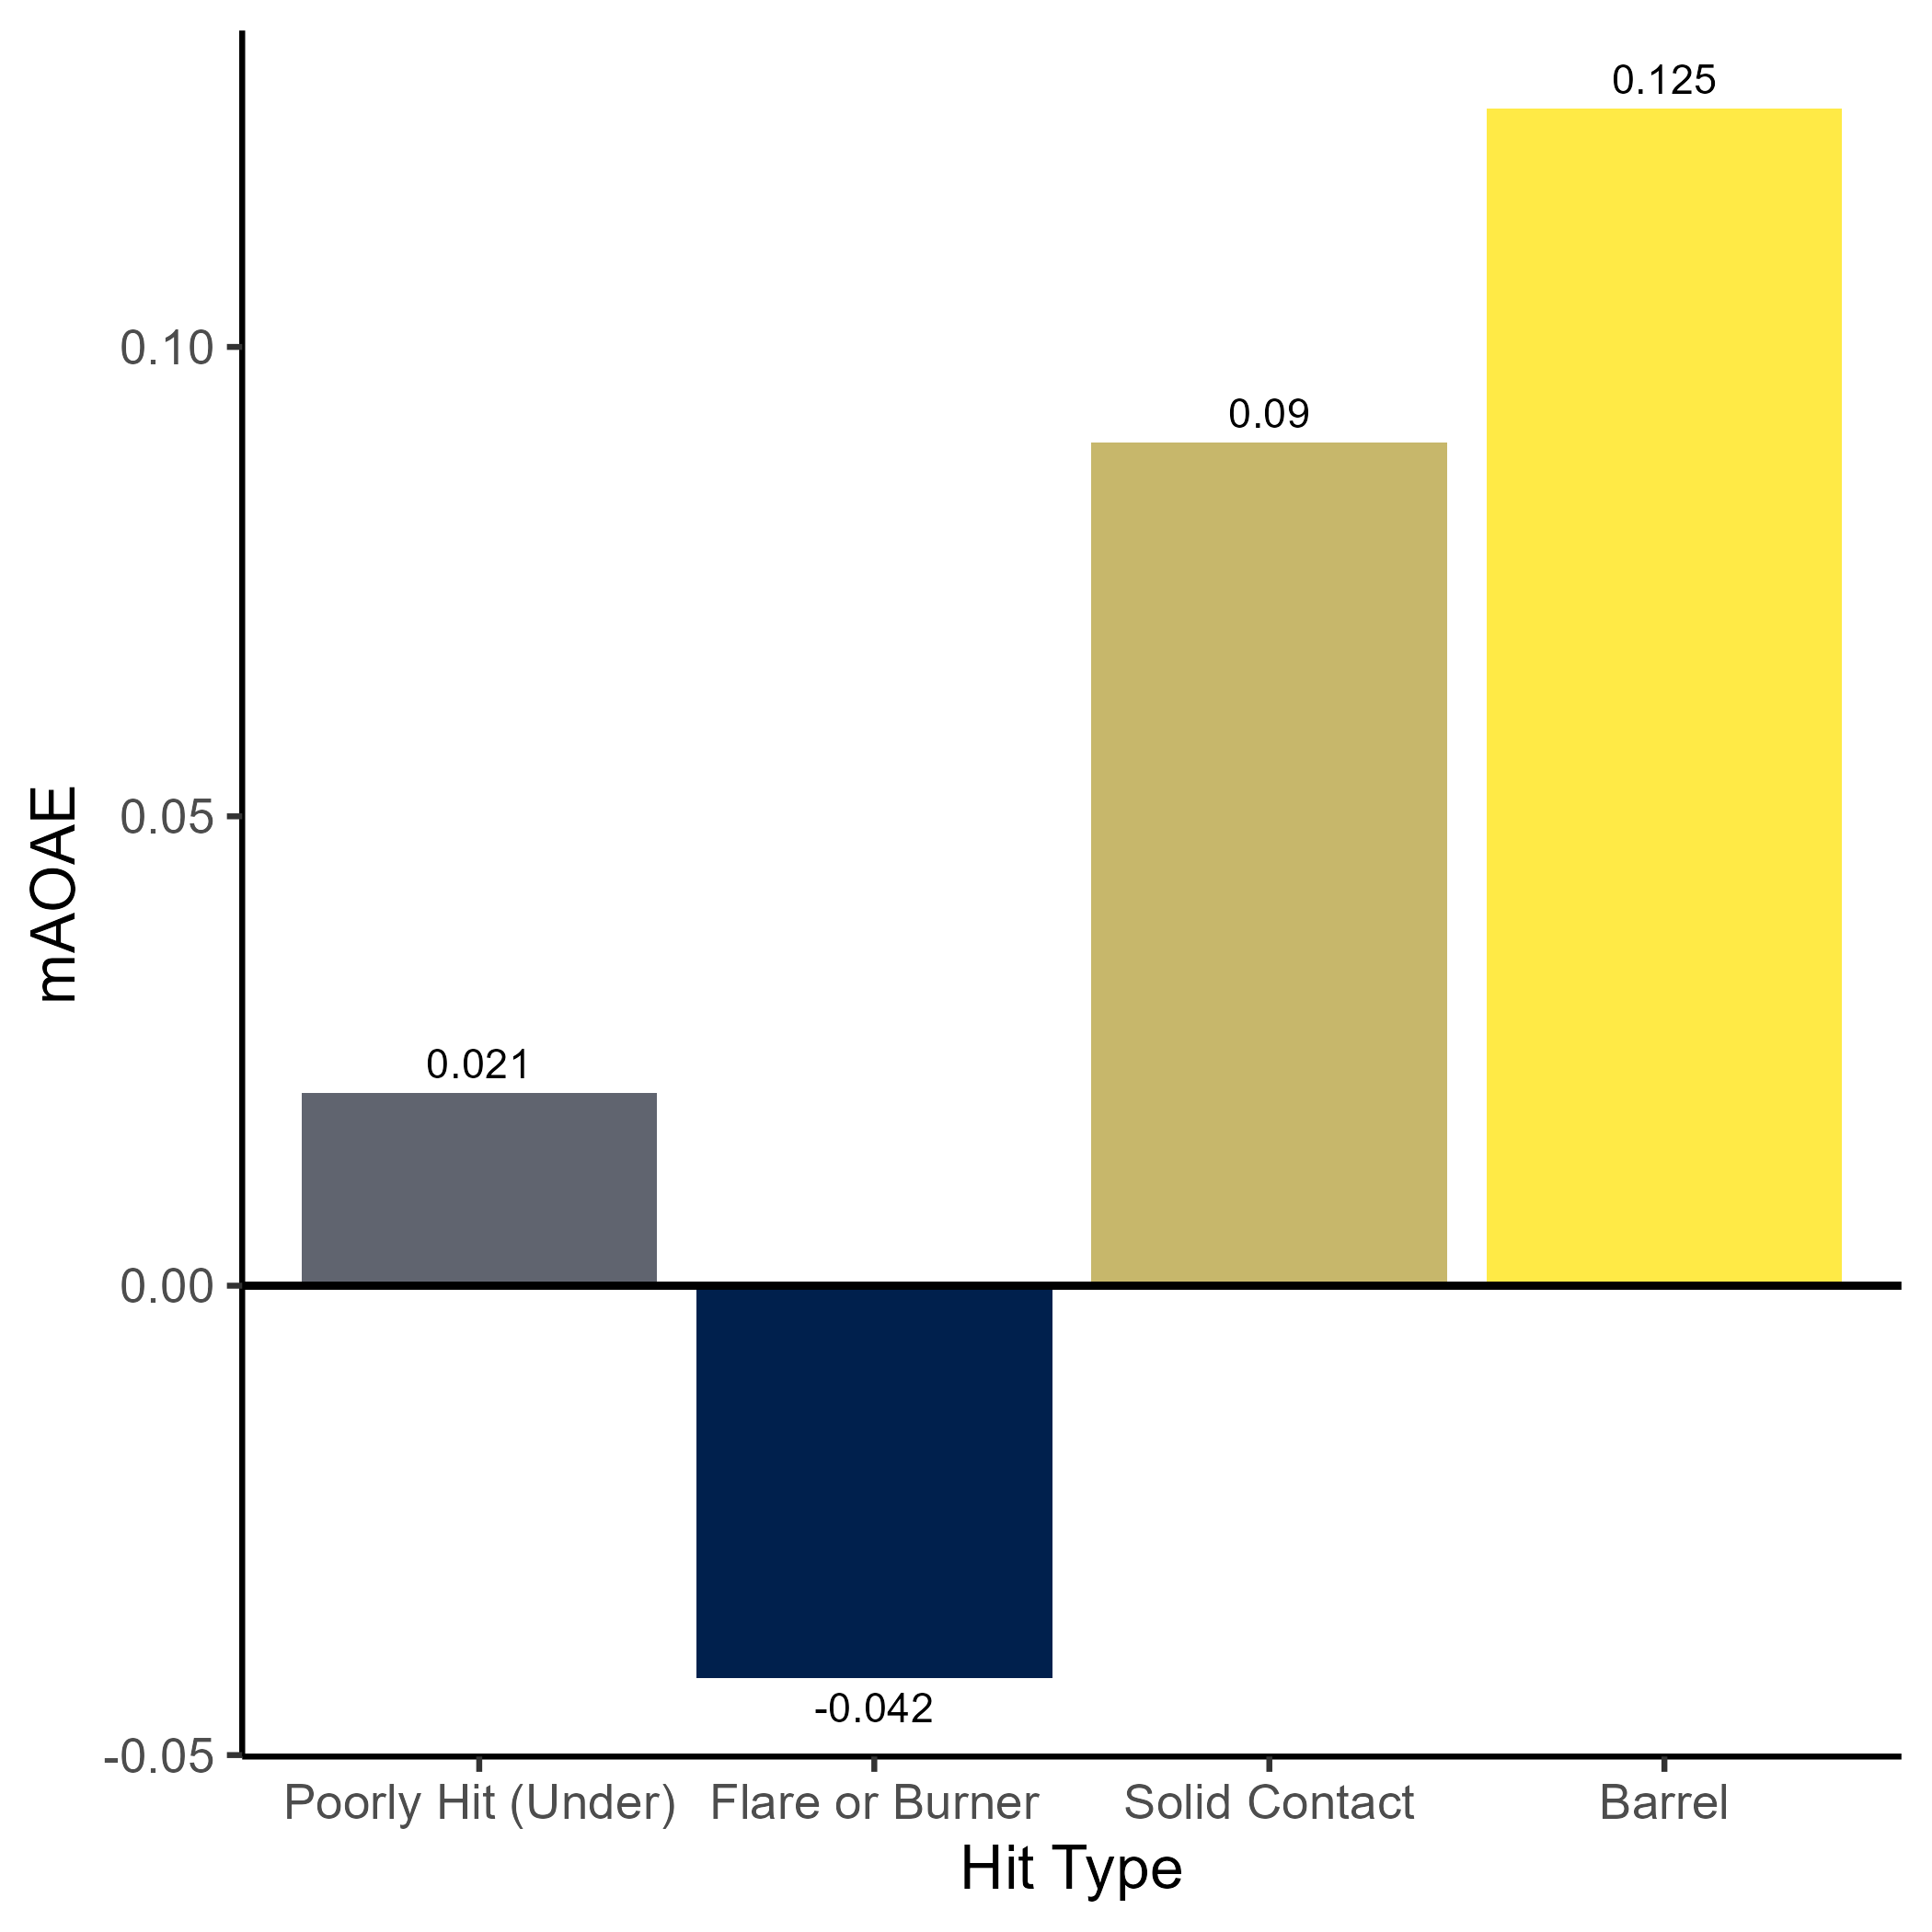
\includegraphics[width = 0.47\textwidth]{../../output/figs/hit_type_15411.png}
    \caption{Player 15411's Fielding Performance Against Hit Type}
    \label{fig:hittype}
  \end{figure}

  TODO: Explain hit types, reference article

\subsection{Adjustment to Level A}
\label{sec:adjustment}

